\section{Take-Away}
\begin{frame}{Take-Away}
	\begin{columns}
		\begin{column}{0.75\textwidth}
			\begin{itemize}
				\item Spark basiert auf der Idee von schreibgeschützten, verteilten Datensätzen
				\item RDDs können mit diversen Transformationen und Aktionen verarbeitet werden
				\item Aufwändige Transformationen können durch Lazy-Evaluation optimiert werden
				\item Fehlertoleranz wird durch simples Neuberechnen erzeugt
				\item Zusätzliche APIs für weitere Anwendungsfälle
			\end{itemize}
		\end{column}
		\begin{column}{0.25\textwidth}
			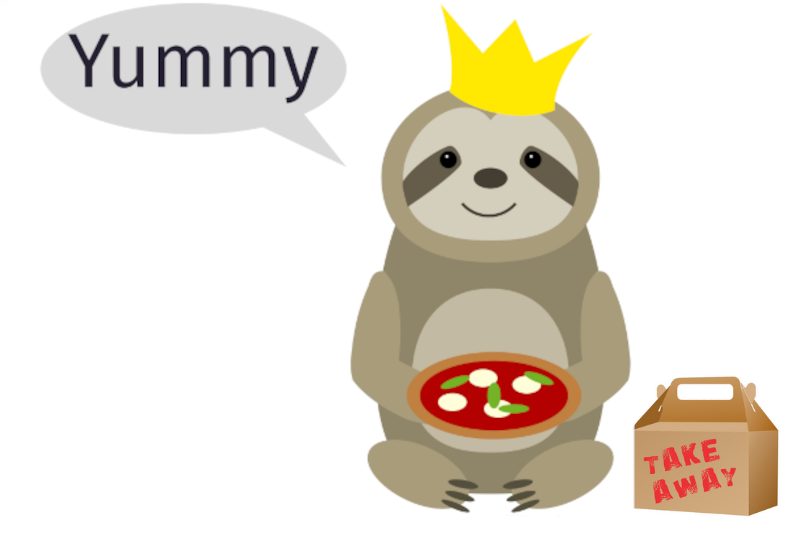
\includegraphics[width=\textwidth]{pics/sloth.png}\\
		\end{column}
	\end{columns}
\end{frame}
